\section{Results}\label{sec:results}

The Friedman Test showed no significant difference in values among tournament size values across all functions. The test was repeated for dimensions: 10, 20 and 40 dimensions and similar results were found. Detailed data can be visualized on the following Table~\ref{Friedman_test}. 

\vspace{3mm}
\begin{table}[h]
	\centering
	\begin{tabular}{|l|l|l|}
		\hline
		Dimension size      & Chi-squared        & P-value                     \\ \hline
		\multicolumn{1}{|l|}{10} & \multicolumn{1}{l|}{31.497} & \multicolumn{1}{l|}{0.1111} \\ \hline
		\multicolumn{1}{|l|}{20} & \multicolumn{1}{l|}{27.903} & \multicolumn{1}{l|}{0.2195} \\ \hline
		\multicolumn{1}{|l|}{40} & \multicolumn{1}{l|}{23.288} & \multicolumn{1}{l|}{0.444}  \\ \hline
	\end{tabular}
	\caption{Friedman Test results.}
	\label{Friedman_test}	
\end{table}


\begin{figure*}[t]
	\begin{subfigure}[b]{0.33\textwidth}
		\centering
		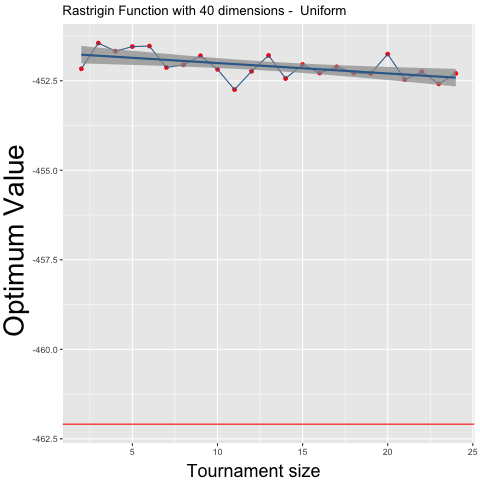
\includegraphics[width=\textwidth]{img/multimodal_uniform_3_dim_40.png}
		\caption{10 dimensions.}
	\end{subfigure}
	\begin{subfigure}[b]{0.33\textwidth}
		\centering
		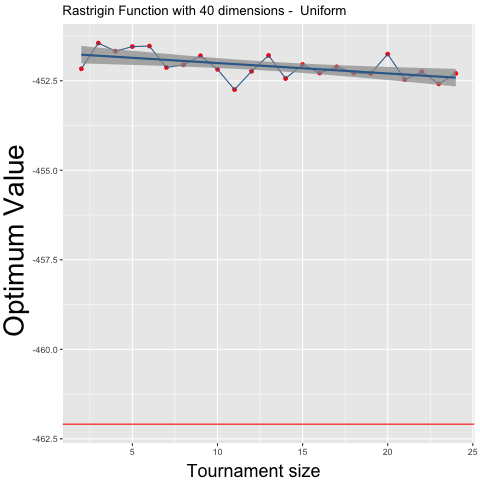
\includegraphics[width=\textwidth]{img/multimodal_uniform_3_dim_40.png}
		\caption{20 dimensions.}
	\end{subfigure}
	\begin{subfigure}[b]{0.33\textwidth}
		\centering
		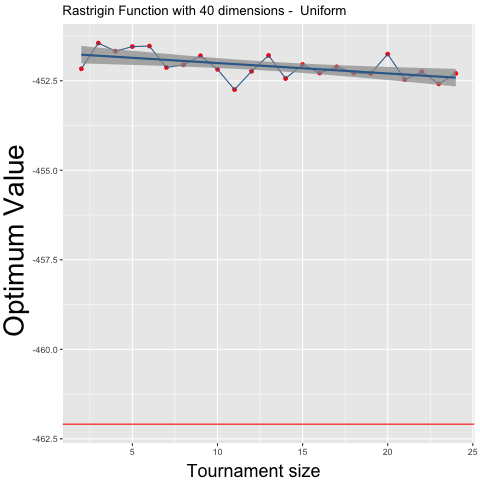
\includegraphics[width=\textwidth]{img/multimodal_uniform_3_dim_40.png}
		\caption{40 dimensions.}
	\end{subfigure}
	\caption{Average performance on different tournament size for the F5 function.}
	\label{5}
\end{figure*}

\begin{figure*}[t]
	\begin{subfigure}[b]{0.33\textwidth}
		\centering
		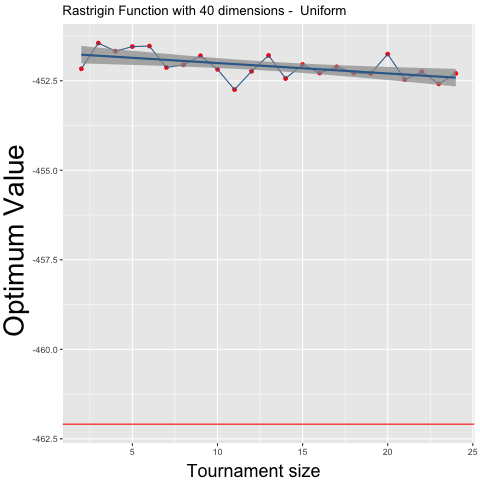
\includegraphics[width=\textwidth]{img/multimodal_uniform_3_dim_40.png}
		\caption{10 dimensions.}
	\end{subfigure}
	\begin{subfigure}[b]{0.33\textwidth}
		\centering
		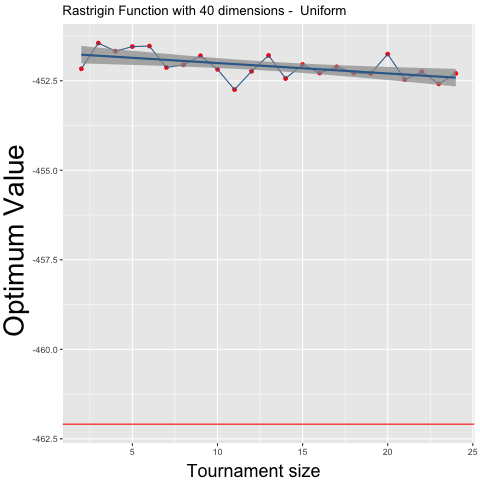
\includegraphics[width=\textwidth]{img/multimodal_uniform_3_dim_40.png}
		\caption{20 dimensions.}
	\end{subfigure}
	\begin{subfigure}[b]{0.33\textwidth}
		\centering
		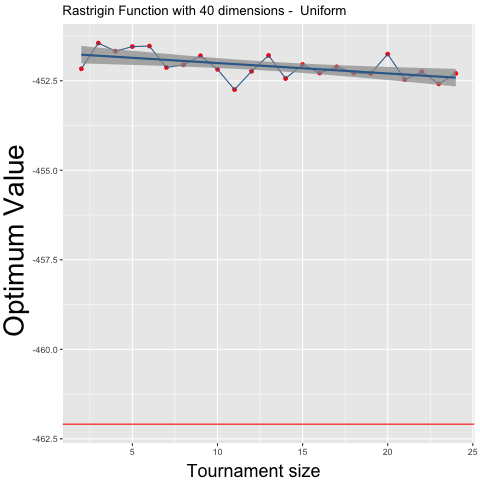
\includegraphics[width=\textwidth]{img/multimodal_uniform_3_dim_40.png}
		\caption{40 dimensions.}
	\end{subfigure}
	\caption{Average performance on different tournament size for the F12 function.}
	\label{12}
\end{figure*}


\begin{figure*}[t]
	\begin{subfigure}[b]{0.33\textwidth}
		\centering
		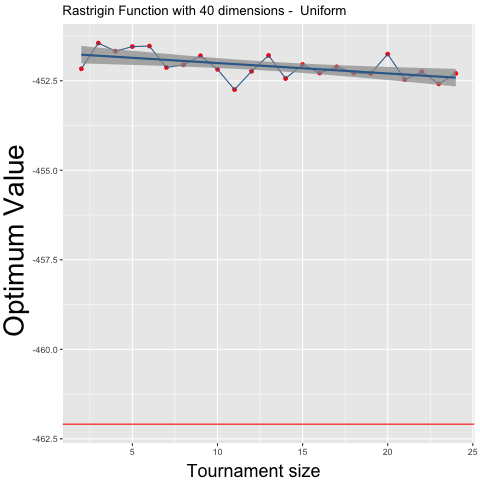
\includegraphics[width=\textwidth]{img/multimodal_uniform_3_dim_40.png}
		\caption{10 dimensions.}
	\end{subfigure}
	\begin{subfigure}[b]{0.33\textwidth}
		\centering
		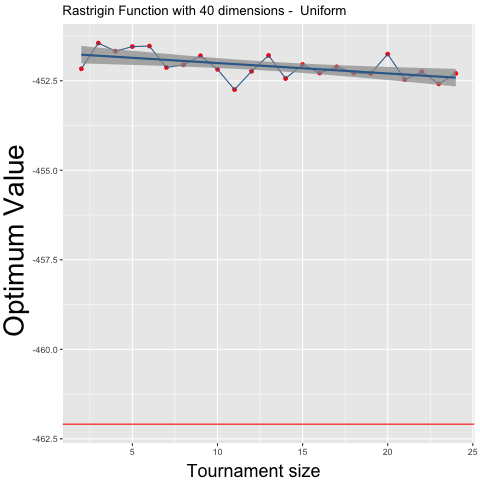
\includegraphics[width=\textwidth]{img/multimodal_uniform_3_dim_40.png}
		\caption{20 dimensions.}
	\end{subfigure}
	\begin{subfigure}[b]{0.33\textwidth}
		\centering
		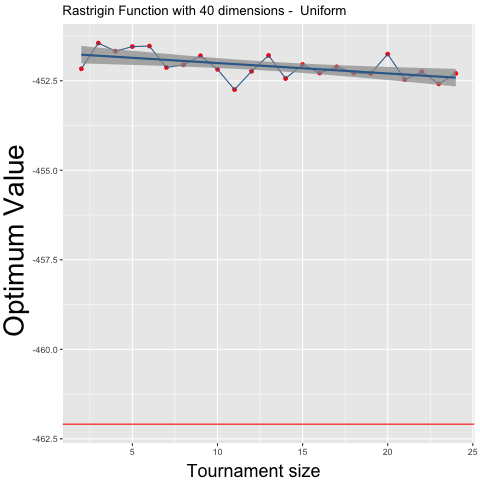
\includegraphics[width=\textwidth]{img/multimodal_uniform_3_dim_40.png}
		\caption{40 dimensions.}
	\end{subfigure}
	\caption{Average performance on different tournament size for the F21 function.}
	\label{21}
\end{figure*}


To get a finer intuition about the results, we show  some visual examples, separated in two groups of Figures. The first group, shows the mean value achieved by the GA given a function. The second one, shows the convergence plot with the mean of the values found at each generation, the function target value with a given tournament size.

All Figures represent the mean of 34 repetitions given a certain dimension.

%To better understand the results, we performed the Friedman Test over all optimum values found from the GA.% These optimum values represent the values obtained from the 1728 different combinations paired by the 24 functions, the 3 dimensions and the 24 tournament sizes.




\subsection{Tournament Size by Functions Analysis}
The Figures~\ref{5},~\ref{12},~\ref{21} exemplify that for the F5, F12, and F21 function (with 10, 20 and 40 dimensions) that changing the tournament size does not lead to significant better final values found by the GA. The gray shaded area represents the 95\% confidence level interval for predictions from a linear model for each scenario showed and demonstrate that no value of the tournament size has consistently better results. For all Figures, the mean of 34 repetitions is shown as bullets and the bars represent the standard deviation, with 40 dimensions. 

